\documentclass[titlepage]{article}
\title{Tietokantojen perusteiden ryhm\"aty\"o - keskustelupalsta}
\author{Valtteri Eskola 014471751, \\ Anne Kiirikki 014420773, \\ Joel Petro 014428047, \\ Vesa Riekkinen 013613345}
\date{}

\usepackage[utf8]{inputenc}
\usepackage[T1]{fontenc}
\usepackage[finnish]{babel}
\usepackage{graphicx}
\usepackage{float}
\usepackage{hyperref} 

\begin{document}
\maketitle

\noindent \textbf{Web-sovelluksen osoite:} \href{
http://keskustelupalsta.herokuapp.com/}{
http://keskustelupalsta.herokuapp.com/} \\
\noindent Keskustelupalstalla voi luoda uusia aihealueita, luoda uusia keskusteluja ja vastata keskusteluketjuihin.\\

\noindent \textbf{Web-sovelluksen koodit:} \href{https://github.com/vesarie/palsta}{https://github.com/vesarie/palsta}

\section*{Käsitekaavio}
Tarpeelliset käsitteet keskustelupalstan luomiseksi  ovat alue, keskustelu ja viesti. Kuvassa \ref{käsite} näkyvät niiden väliset osallitumisrajoitteet ja riippuvuudet.

\begin{figure}[H]
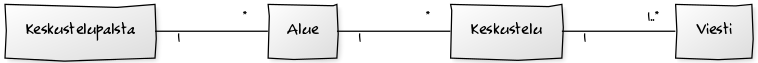
\includegraphics[width=\textwidth]{kasitekaavio}
\label{käsite}
\caption{Keskustelupalstan osallistumisrajoitteet}
\end{figure}

\section*{Attribuutit}

\noindent Taulukossa on listattu kunkin taulun tarvitsemat attribuutit ja avaimet. \\

{
\centering
\begin{tabular}[width=\textwidth]{r|l}

Käsite & Attribuutit \\
\hline
Alue & (pk) tunnus integer, nimi varchar(), web{\_}tunnus varchar(n) \\
Keskustelu & (pk) tunnus integer , (fk) alue : Alue,  otsikko varchar(n) \\
Viesti & (pk) tunnus, (fk) keskustelu : Keskustelu, pvm TIMESTAMP, \\
& sisalto varchar(n) \\
\end{tabular}
} \\

\section*{Tietokantakaavio}

\begin{figure}[H]
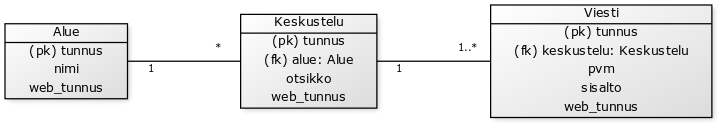
\includegraphics[width=\textwidth]{tietokantakaavio}
\label{tkkaavio}
\caption{Tietokantakaavio}
\end{figure}

\section*{Taulujen luonti SQL-komennoilla}

CREATE TABLE Alue ( 
\begin{itemize}
	\item[] tunnus integer PRIMARY KEY,
    \item[] web{\_}tunnus varchar(100) NOT NULL UNIQUE,
    \item[] nimi varchar(100) NOT NULL,
\end{itemize}
); \\

\noindent CREATE TABLE Keskustelu ( 
\begin{itemize}
	\item[] tunnus integer PRIMARY KEY,
    \item[] alue integer NOT NULL,
    \item[] web{\_}tunnus integer NOT NULL UNIQUE,
    \item[] otsikko varchar(250) NOT NULL,
    \item[] FOREIGN KEY(alue) REFERENCES Alue(tunnus)

\end{itemize}
); \\

\noindent CREATE TABLE Viesti ( 
\begin{itemize}
	\item[] tunnus integer PRIMARY KEY,
    \item[] keskustelu integer NOT NULL,
    \item[] lahettaja varchar(100) NOT NULL,
    \item[] pvm TIMESTAMP NOT NULL,
    \item[] web{\_}tunnus integer NOT NULL,
    \item[] sisalto text NOT NULL,
    \item[] FOREIGN KEY(keskustelu) REFERENCES Keskustelu(tunnus)


\end{itemize}
); \\


\section*{Muutamia olennaisia käyttötapauksia}

\subsection*{Alueiden listaus}

SELECT a.nimi, COUNT(v.tunnus) AS viesteja, \\ MAX(v.pvm) AS viimeisin 
FROM Alue a
\begin{itemize}
	\item[] LEFT JOIN Keskustelu k ON a.tunnus = k.alue
    \item[] LEFT JOIN Viesti v ON k.tunnus = v.keskustelu
\end{itemize}
GROUP BY a.tunnus
ORDER BY a.nimi \\

\noindent
Komennossa haetaan kaikki alueet, niiden sisältämien viestien lukumäärä ja uusimman viestin lähetysaika. Komennon suorittamiseen tarvitaan tietoa kolmesta eri talulusta: Alue, Keskustelu ja Viesti. Samalla lasketaan myös viestien määrä aihealueittain ja viimeisimmän viestin lähetysaika. Listaus on ryhmitelty alueen tunnuksen perusteella ja aakkosjärjestyksessä alueen nimen mukaan. Koodissa komento on jaettu kahdeksi eri metodiksi, mutta yhdessä ne näyttävät tältä. 

\subsection*{Alueen sisältämien keskustelujen listaaminen}

Kun halutaan saada selville alueen sisältämät keskustelut tarvitaan tietoa tauluista Alue, Keskustelu ja Viesti.\\

\noindent SELECT k.otsikko AS keskustelu, COUNT(v.tunnus) AS viesteja, \\ MAX(v.pvm) AS viimeisin 
FROM Alue a
\begin{itemize}
  \item[] INNER JOIN Keskustelu k ON a.tunnus = k.alue
  \item[] LEFT JOIN Viesti v ON k.tunnus = v.keskustelu
\end{itemize}
WHERE alue.web{\_}tunnus = ? \\
GROUP BY k.tunnus \\
ORDER BY viimeisin DESC \\
LIMIT 10 OFFSET ? \\

\noindent Kysely listaa kymmenen tuoreinta keskustelua viimeisimmän viestin perusteella ja kunkin keskustelun viestien lukumäärän. Samalla lasketaan keskustelun sisältämien viestien määrä ja viimeisimmän viestin lähetysaika. 


\subsection*{Viestin lisääminen}

\noindent Kun käyttäjä lähettää viestin, hän syöttää yhteen kenttään nimimerkkinsä ja toiseen viestin sisällön. Keskustelun tunnus yhdistää viestin oikeaan keskusteluun ja se selvitetään automaattisesti ohjelman puolesta. Myös päivämäärä luodaan automaatisesti.\\

\noindent INSERT INTO Viesti (keskustelu, lahettaja, pvm, sisalto) VALUES (?,?); \\

\noindent Uutta viestiä lisättäessä tarvitaan keskustelun tunnus, lähettäjän nimimerkki, aika ja viestin sisältö Kysymysmerkit viittaavat keskusteluun, lahettajaan, pvm:ään ja sisaltoon.

\section*{Ongelmia työn toteutuksessa}

\noindent Sovelluksen siirtäminen Herokuun tuotti hieman ongelmia. Kansiorakennetta piti muuttaa siten, että Netbeans-projekti siirrettiin alikansiosta Git-repositorion juureen. Ilman tätä projekti ei kääntynyt Herokun palvelimella, koska “buildpack” ei löytänyt projektia. Tämä on puhtaasti “buildpackin” asettama rajoitus.

Myös joihinkin kyselyihin piti tehdä vähäisiä tarkennuksia, koska PostgreSQL oli kyselyiden suhteen tarkempi. Yhteen findOne-tyyppiseen kyselyyn piti lisätä GROUP BY -määre, jolla ei ollut vaikutusta lopputulokseen.

Uuden keskustelun lisääminen tietokantaan oli toinen esimerkki, jossa jouduttiin tekemään hieman töitä sen kanssa, että keksittiin ratkaisu, joka toimii sekä SQLitessa että PostgreSQL:ssä. Ilmeisesti standardi SQL ei tarjoa helppoa keinoa INSERT-kyselyn luoman pääavaimen (eli tässä tapauksessa keskustelun tunnuksen) palauttamiseen. Onneksi JDBC tarjoaa ratkaisun, joka hyödyntää kullakin tietokanta-alustalla kunkin alustan omaa ratkaisua. Javan tietokantarajapinta JDBC tarjoaa tätä varten metodin getGeneratedKeys (versiosta 3 alkaen).

Myös päivämäärien käsittelyä jouduttiin miettimään. Kuten tiedetään SQLitessa ei ole erillistä timestamp-tyyppiä toisin kuin Herokun tarjoamassa Postgre-SQL:ssä. Käytännössä tämä ilmeni esimerkiksi sillä tavalla, että ResultSetin metodi getTimestamp ei toiminut odotetulla tavalla. Ongelma ratkaistiin tekemällä luokka DateHelper, joka abstrahoi päivämäärien lukemisen kannasta ja kirjoittamisen kantaan. SQLiten tapauksessa aikaleimat tallennetaan merkkijonoina. Taulujen määrittelyissä käytettiin silti standardia timestamp-tyyppiä.

Herokun palvelimen kello vaikuttaisi olevan UTC-ajassa, eli talvella 2 tuntia Suomen aikaa jäljessä. Uusien viestien aikaleimat siis olivat aluksi 2 tuntia jäljessä. Ratkaisu oli Heroku Toolbeltin komento heroku config:add TZ="Europe/Hel-sinki”


\section*{Jatkokehitysmahdollisuuksia}

Keskutelupalstaa voisi hienosäätää esimerkiksi siten, että käyttäjä voisi kirjautua sisään tunnuksella ja salasanalla. Viestien lisäystä voisi monipuolistaa luomalla mahdollisuuden lisätä linkkejä, kuvia ja lainata toisten käyttäjien viestejä. Keskustelupalstalle voisi lisätä hakuominaisuuden ja pakollisen "Jaa Facebookissa" -napin. Sivuston ulkoasu voisi olla kauniimpi. Navigointipalkki voisi helpottaa sivustolla liikkumista. Keskustelut, joihin on tullut uusia viestejä, voisivat näkyä korostetusti käyttäjälle. Nettirikollisuuden kitkemiseksi tarvitaan Nettivinkki-pikalinkki 

\end{document}



































